\documentclass{article}
\usepackage[utf8]{inputenc}
\usepackage[a4paper, total={6in, 8in}]{geometry}

\title{SPROJ: My Permanent Existential Crisis}
\author{Derek Low}
\date{2017-2018}

\usepackage{natbib}
\usepackage{graphicx}
\renewcommand{\baselinestretch}{1.6}
\begin{document}

\section{Methods}
\subsection{Simulation of Neurons for Spike Train Generation}
The NEST simulator is used for the purposes of generating spike train data. NEST Izhikevich neurons are used as the model neurons, due to the increased complexity over leaky integrate-and-fire neurons, and the reduced computational complexity over models of significantly more numerous compartment models, such as the Hodgkin-Huxley models (Brette, 2015). NEST implementation dynamics of Izchikevich neurons are provided by the following :

$$dv/dt=0.04v^2+5v+140-u+I$$
$$du/dt=a(bv-u)$$

$$if v >= V_th:{$$
\tab$$v = c$$
\tab$$u = u + d}$$$

where $v$ represents the membrane potential of the neuron and $u$ the membrane recovery variable. The membrane recovery variable captures the responses of $K^{+}$ and $Na^{+}$, and is a source of negative feedback to $v$. Coefficients for change in membrane potential, are based on scale, with membrane potential at $mV$ and time as ms, as are $a$ and $b$. $I$ is the input current to the neuron, and $c$ and $d$ are the post-spike reset values of the neuron (Kunkel et al., 2017, Izhikevich et al., 2004). 

To simulate a population of neurons with $n$ population size over $t$ time, a file containing an $n x n$ adjacency matrix is provided to the simulation program, which then creates a NEST neuron population with the exact number of neurons and connections between the neurons in the population, using the corresponding weight of the connection stored in the adjacency matrix. Interactions with neurons in NEST must be achieved through the creation of new node objects, made to represent and achieve the results of physical instruments and devices; therefore, we create a poisson generator node to add noise to the population, and connect a spike detector node to record all spikes in the population during simulation. The population is then recorded over 1000 simulation steps, or 100 ms. The corresposnding output of the simulation is converted to a matrix of $n x t$ dimensionality.\par

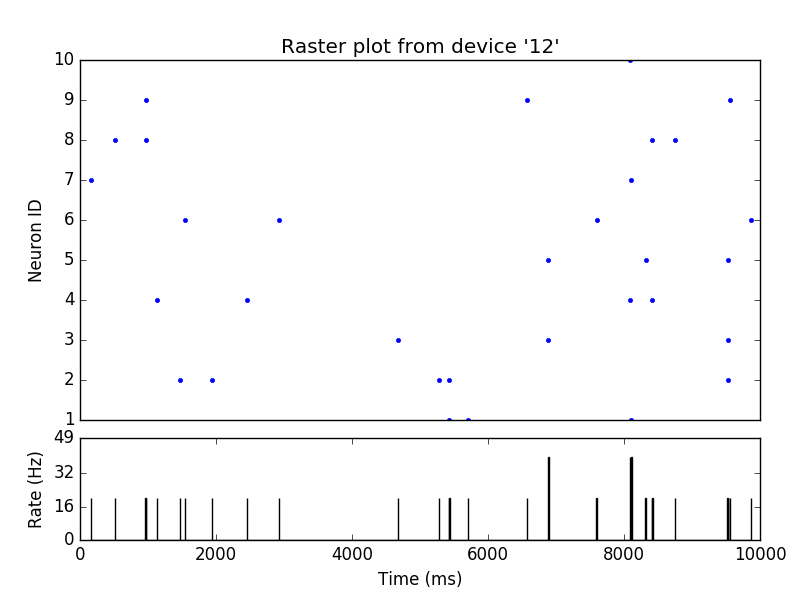
\includegraphics[scale=0.5]{figures/figure1.png} 

\subsection{PageRank}
The PageRank-based algorithm takes a weighted adjacency matrix as an input; a non-weighted adjacency matrix would result in no change in the PageRanks of each neuron, and no change in the resulting adjacency matrix. The PageRank for each neuron is then calculated based on the following formula:

$$PR_i = (1-d)+d(\sum(\frac{PR_j}{C} * W_ij))$$

Where PR is the PageRank of neuron $i$, $d$ is the standard damping factor of 0.8, $PR_j$ is the PageRank of incoming neuron j, and $W_j_i$ is the weight of the connection from neuron j to i. The summation calculates for all incoming connections to neuron i. The formula is recalculated until convergence, where the PageRanks no longer change, at which point the weights are updated such that the weight of each connection is multiplied by the PageRank of the source of the connection. The network is then pruned by comparing the weights between neuron i and j, or Wij and Wji, and the the lower value is reduced to 0, while the higher value is set to 1, preserving the higher connection. The process is then repeated, using the new weights, for an arbitrary number of times.\par



\end{document}